\documentclass{article}
\usepackage[T1]{fontenc}
\usepackage{lmodern}
\usepackage{graphicx}
\usepackage{amsmath,amssymb}
\usepackage[a4paper,margin=2cm]{geometry}
\usepackage[absolute,overlay]{textpos}
\setlength{\TPHorizModule}{1mm}
\setlength{\TPVertModule}{1mm}
\usepackage[indonesian]{babel}
\usepackage{hyperref}
\setlength{\emergencystretch}{2em}
% unit: Halaman 3

\begin{document}

% === Halaman 3 (python/native) ===

3

• Cipher di dalam kriptografi klasik disusun oleh dua teknik dasar:

1. Teknik substitusi: mengganti huruf plainteks dengan huruf cipherteks.


        Contoh:     Plainteks:    MENGANTUK 



       Cipherteks: CQBSIBONW

2.

Teknik transposisi: mengubah susunan atau posisi huruf plainteks menjadi 

susunan huruf cipherteks. 


  Disebut juga teknik scrambling, permutasi, atau pengacakan 


 Contoh:     Plainteks:    MENGANTUK 



       Cipherteks: TNEAKMNGU

Plainteks:

Cipherteks:

% deskripsi: gambar native xref 35
\noindent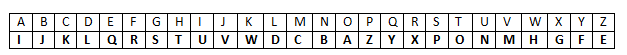
\includegraphics[width=0.85\textwidth]{../../images/python/page_003_img_01.png}

\end{document}
